% Digital Logic Report Template
% Created: 2020-01-10, John Miller

%==========================================================
%=========== Document Setup  ==============================

% Formatting defined by class file
\documentclass[11pt]{article}

% ---- Document formatting ----
\usepackage[margin=1in]{geometry}	% Narrower margins
\usepackage{booktabs}				% Nice formatting of tables
\usepackage{graphicx}				% Ability to include graphics
\usepackage[section]{placeins}      % Stops floats from happening

%\setlength\parindent{0pt}	% Do not indent first line of paragraphs 
\usepackage[parfill]{parskip}		% Line space b/w paragraphs
%	parfill option prevents last line of pgrph from being fully justified

% Parskip package adds too much space around titles, fix with this
\RequirePackage{titlesec}
\titlespacing\section{0pt}{8pt plus 4pt minus 2pt}{3pt plus 2pt minus 2pt}
\titlespacing\subsection{0pt}{4pt plus 4pt minus 2pt}{-2pt plus 2pt minus 2pt}
\titlespacing\subsubsection{0pt}{2pt plus 4pt minus 2pt}{-6pt plus 2pt minus 2pt}

% ---- Hyperlinks ----
\usepackage[colorlinks=true,urlcolor=blue]{hyperref}	% For URL's. Automatically links internal references.

% ---- Code listings ----
\usepackage{listings} 					% Nice code layout and inclusion
\usepackage[usenames,dvipsnames]{xcolor}	% Colors (needs to be defined before using colors)

% Define custom colors for listings
\definecolor{listinggray}{gray}{0.98}		% Listings background color
\definecolor{rulegray}{gray}{0.7}			% Listings rule/frame color

% Style for Verilog
\lstdefinestyle{Verilog}{
	language=Verilog,					% Verilog
	backgroundcolor=\color{listinggray},	% light gray background
	rulecolor=\color{blue}, 			% blue frame lines
	frame=tb,							% lines above & below
	linewidth=\columnwidth, 			% set line width
	basicstyle=\small\ttfamily,	% basic font style that is used for the code	
	breaklines=true, 					% allow breaking across columns/pages
	tabsize=3,							% set tab size
	commentstyle=\color{gray},	% comments in italic 
	stringstyle=\upshape,				% strings are printed in normal font
	showspaces=false,					% don't underscore spaces
}

% How to use: \Verilog[listing_options]{file}
\newcommand{\Verilog}[2][]{%
	\lstinputlisting[style=Verilog,#1]{#2}
}




%======================================================
%=========== Body  ====================================
\begin{document}

\title{ELC 2137 Lab 11: FSM: Guessing Game}
\author{Maddie Vorhies}

\maketitle


\section*{Summary}

The goal of this lab is to use what we have learned in previous labs to create a guessing game. In order to do this, I first have to create a debounce circuit. A debounce ensures that the value of the input is held for a certain period of time. In this lab we were given the debounce module and the test, so I ran the test just to make sure that I recieved the correct output. In the game, there are two different settings: a fast setting and a slow setting. In order to implement this, I created two seperate counters. Both were very similar, but they have different paramters to distinguish between fast and slow. The larger the parameter the slower the counter so I set my parameter in the fast counter to N = 24 and the slow counter to N = 26. Then  created a mux so that you can choose which setting you ant to play using switch 0. Next, I created a decoder so that the board would display on the upper four segments of the first 7-segment display digit. Lastly I created the guessFSM module which was the guessing game itself. This modules cycles through different states that correspond to different buttons being pressed. If the correct button is pressed at the correct time, you will go to the in state, and if any other button is pressed then you will go to the lose state. After this module was built, I created a testbench to test it. Then I created my overall guessing game module that put all of theses pieces together. I then created a guessing game testbench. Once it was successful I was able to play my game.


\section*{Q\&A}

(a) At what time in the simulation did the debounce circuit reach each of the four states (zero, wait1, one, wait0)? \newline
The simulation starts out in state zero and then reaches wait1 at 200.0ns, then reaches one at about 245.121ns, then reaches wait0 at 600.0ns, and then reaches state zero again at about 646.327ns. \newline 

(b) Why can this game not be implemented with regular sequential logic? \newline
 We can't use regular sequential logic because this game does not have a regular/repeating pattern. In this game, I am using a finite state machine (FSM) which handles irregular, non-repeating conditions. The pattern is non-repeating because we don't know what buttons the user is going to guess and we don't know when they are going to win or lose. They could win twice in a row, then lose one, or lose three times in a row, etc. It is an irregular pattern which means we can't use regular sequential logic. \newline

(c) What type of outputs did you use for your design (Mealy or Moore)? Explain \newline
 For my design, I used Moore because it's a much safer design than Mealy. Mealy is a machine whose ouputs are determined by both its current state and the current inputs. Whereas a Moore machine whose output are only determined by its current state. In a Moore, the outputs only change when the state changes which means that it is synchronized with the clock. In a Mealy, the ouput can change from other inputs as well which means its no longer synchronized with the clock and could cause a glitch. I created a case statement that is only based on the specific states which means that its not based on any other input so it is a Moore machine. 



\section*{Results}

\begin{figure}[ht]\centering
	\caption{Simulation Waveform for Debounce}
	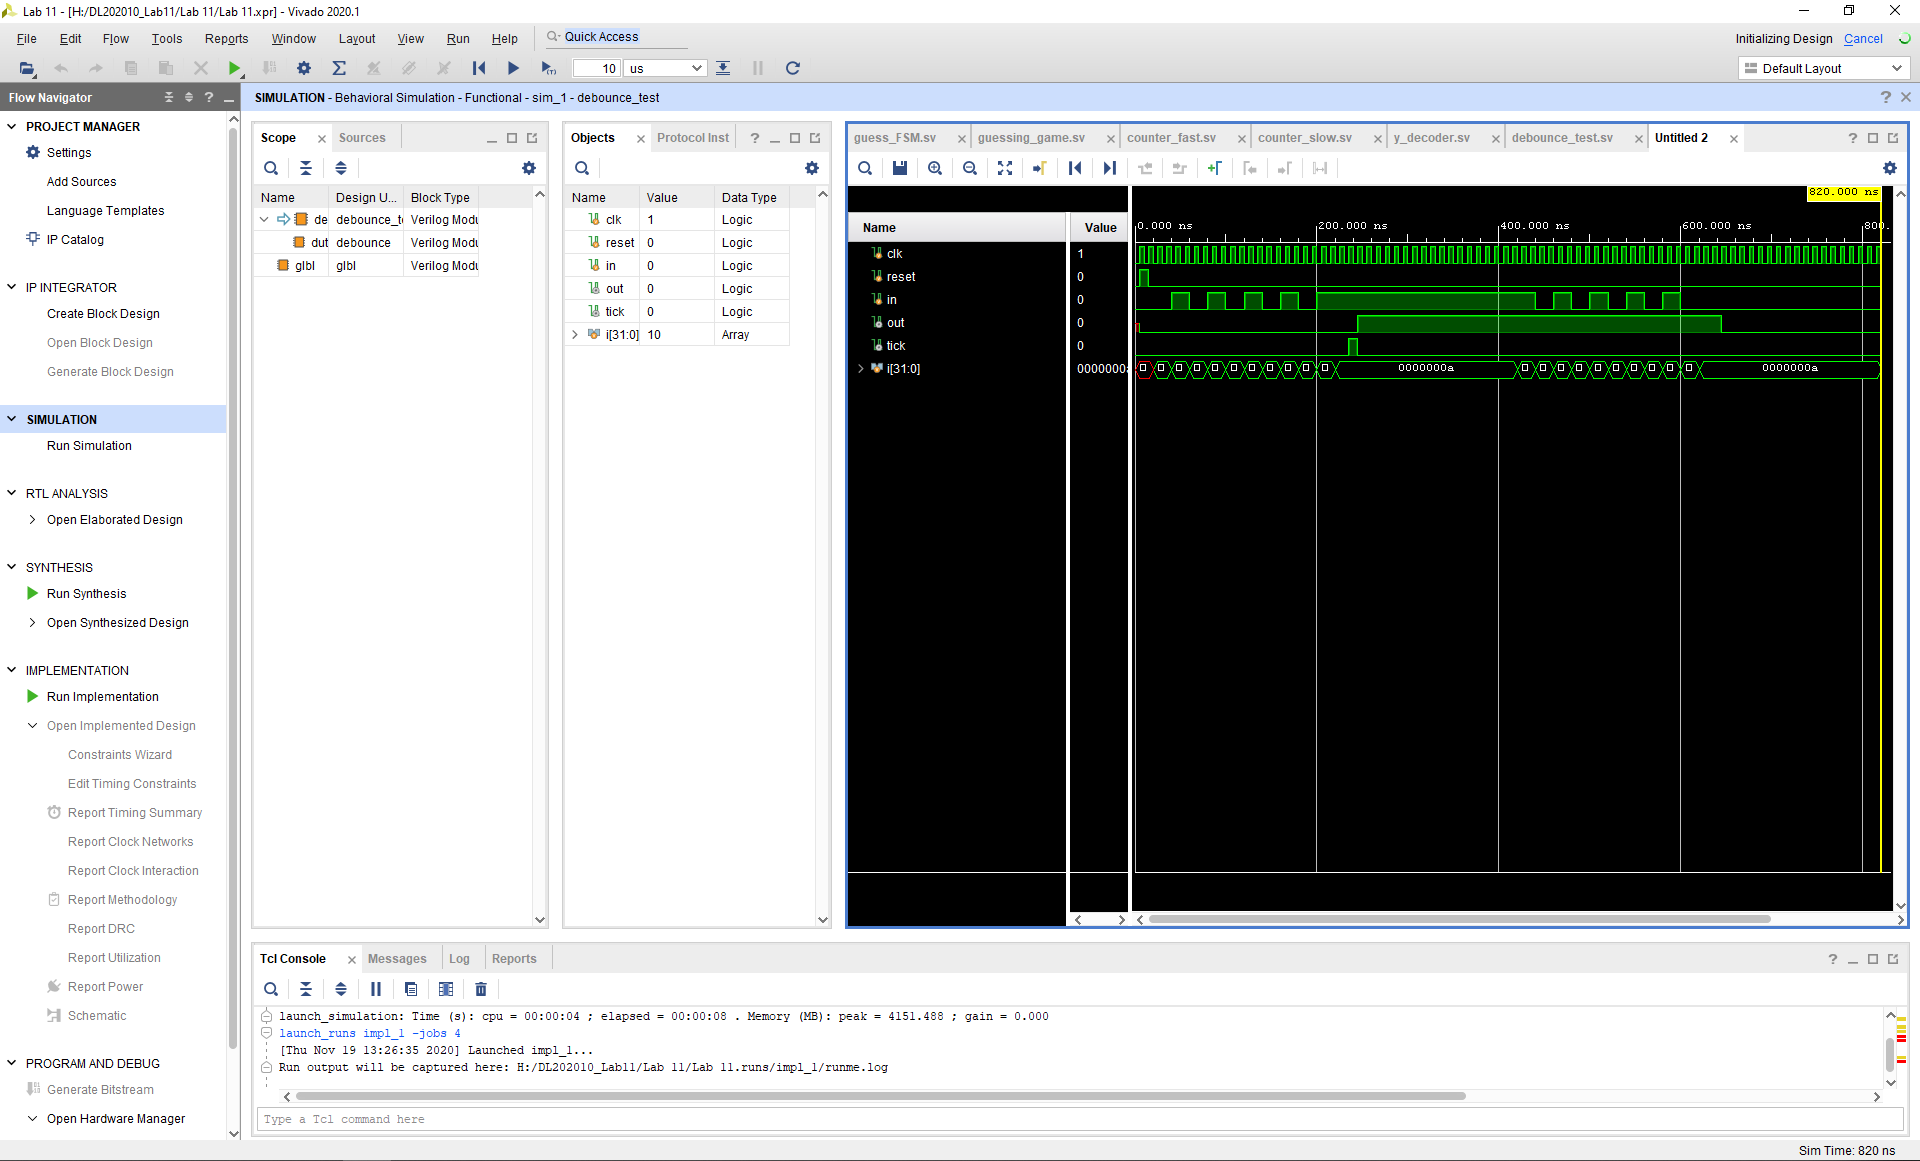
\includegraphics [width=1\textwidth,trim=640 550 10 135, clip]{debounce_sim}
\end{figure}

\begin{figure}[ht]\centering
	\caption{Simulation Waveform for Guess FSM}
	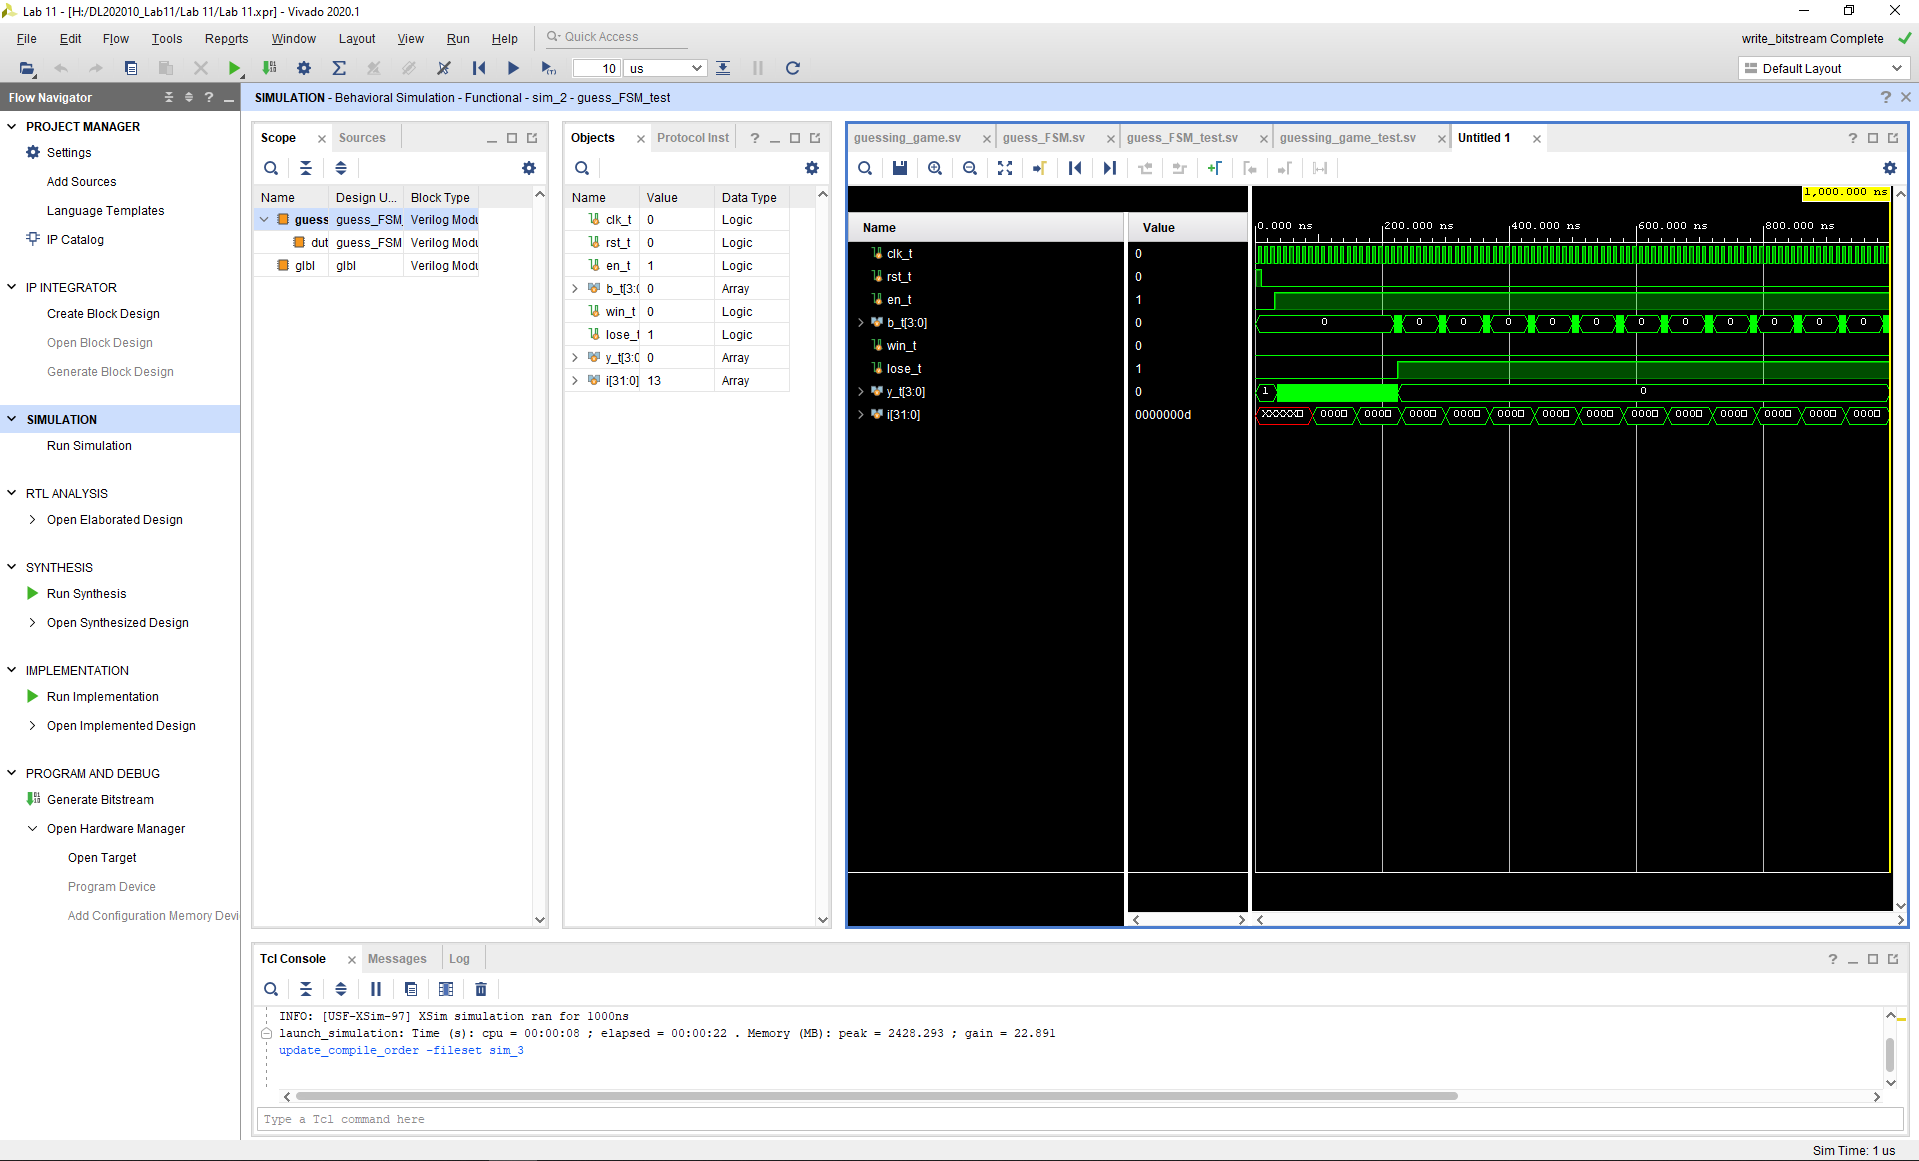
\includegraphics [width=1\textwidth,trim=640 550 10 135, clip]{guess_FSM_sim}
\end{figure}

\begin{figure}[ht]\centering
	\caption{Simulation Waveform for Guessing Game}
	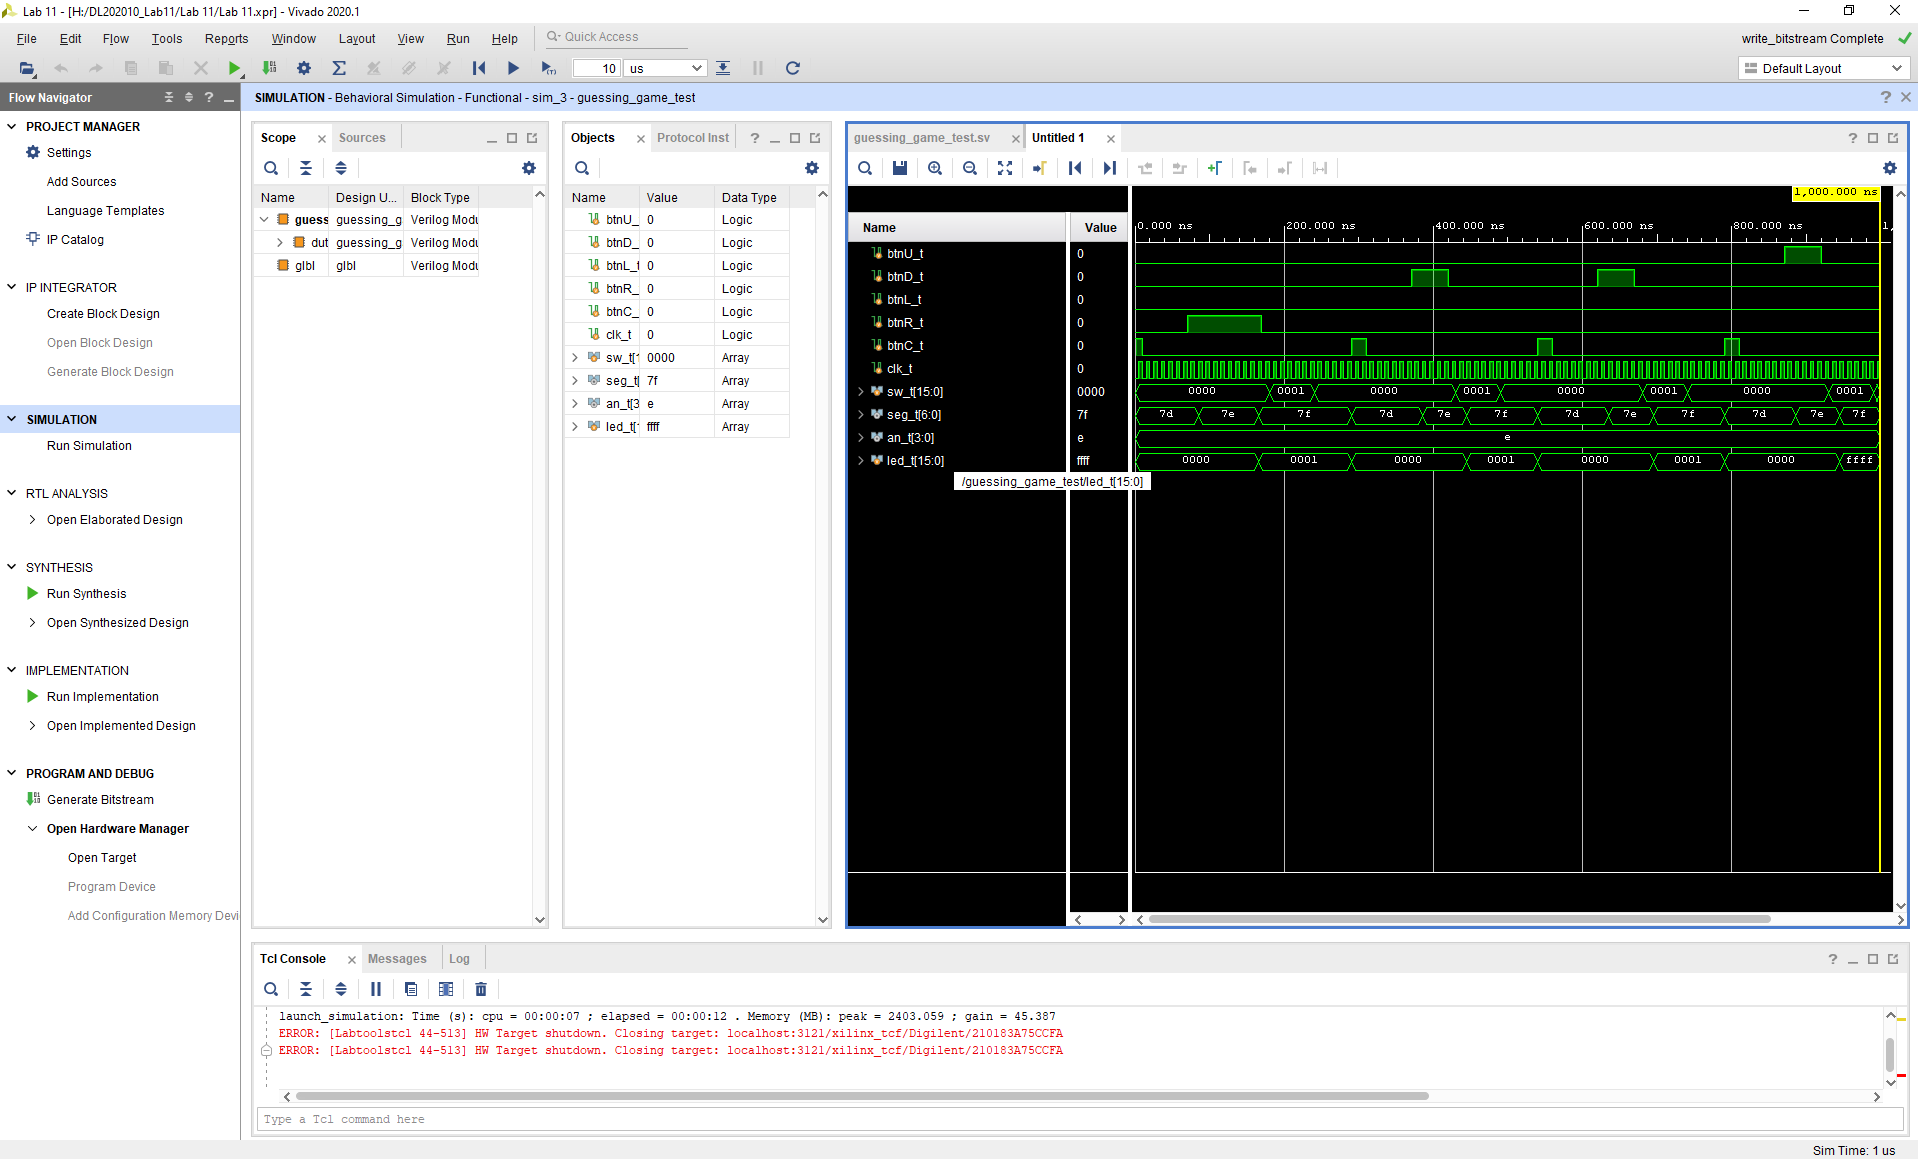
\includegraphics [width=1\textwidth,trim=640 550 10 135, clip]{guessing_game_sim}
\end{figure}

\begin{table*}[ht]\centering
	\caption{10 games on slow setting}
	\label{ALU:tbl:alu_ERT}\medskip
	\begin{tabular}{l|rrrrrrrrrr}
		Game: & 1 & 2 & 3 & 4 & 5 & 6 & 7 & 8 & 9 & 10 \\
		\midrule
		win/lose & win & win & win & lose & win & win & win & win & win & win\\
		segment & right & right & up & down & down & left & left & up & right & down \\
		state & s0 & s0 & s1 & s3 & s3 & s2 & s2 & s1 & s0 & s3\\
		\midrule
		winning percentage & 90 &  &  &  &  & & & & &\\
		\bottomrule
	\end{tabular}
\end{table*}

\begin{table*}[ht]\centering
	\caption{10 games on fast setting}
	\label{ALU:tbl:alu_ERT}\medskip
	\begin{tabular}{l|rrrrrrrrrr}
		Game: & 1 & 2 & 3 & 4 & 5 & 6 & 7 & 8 & 9 & 10 \\
		\midrule
		win/lose & win & win & win & win & win & lose & lose & win & win & win\\
		segment & left & right & left & up & up & right & down & down & up & left \\
		state & s2 & s0 & s2 & s1 & s1 & s0 & s3 & s3 & s1 & s2\\
		\midrule
		winning percentage & 80 &  &  &  &  & & & & &\\
		\bottomrule
	\end{tabular}
\end{table*}

\section*{Code}

\Verilog{Lab11/systemverilog/guess_FSM.sv}

\Verilog{Lab11/systemverilog/guess_FSM_test.sv}

\Verilog{Lab11/systemverilog/guessing_game.sv}

\Verilog{Lab11/systemverilog/guessing_game_test.sv}



\end{document}
